\input{head.inc}
\usepackage{relsize}
\usetikzlibrary{%
    decorations.pathreplacing,%
    decorations.pathmorphing%
}
\usepackage{tikz-3dplot}
\usetikzlibrary{3d}
\usetikzlibrary{intersections}

\makeatletter
\pgfqkeys{/tikz/cs}{
  latitude/.store in=\tikz@cs@latitude,% not needed with '3d' library
  longitude/.style={angle={#1}},% not needed with '3d' library
  theta/.style={latitude={#1}},
  phi/.style={angle={#1}}
}
\tikzdeclarecoordinatesystem{xyz spherical}{% needed even with '3d' library!
  \pgfqkeys{/tikz/cs}{angle=0,radius=0,latitude=0,#1}%
  \pgfpointspherical{\tikz@cs@angle}{\tikz@cs@latitude}{\tikz@cs@xradius}% fix \tikz@cs@radius to \tikz@cs@xradius
}
\makeatother
  
% Präambelbefehle für die Präsentation
\title[TET: Elektromagnetische Wellen X - Reflexion und Brechung]{Elektromagnetische Wellen X - Reflexion und Brechung}

\begin{document}
% 
% Frontmatter 
% 
%%%%%%%%%%%%%%%%%%%%%%%%%%%%%%%%%%%%%%%%%%%%%%%%%%%%%%%%%%%%%%%%%%%%%%%%%%%%%%%%%%%%%%%%%%%%%%%%%%%%%%%%%%%%%%%%%%%%%%%%%%%%% 

%% inserts the title page and the table of contents
\maketitle

% 
% Content 
% 
%%%%%%%%%%%%%%%%%%%%%%%%%%%%%%%%%%%%%%%%%%%%%%%%%%%%%%%%%%%%%%%%%%%%%%%%%%%%%%%%%%%%%%%%%%%%%%%%%%%%%%%%%%%%%%%%%%%%%%%%%%%%% 
\section{Elektromagnetische Wellen X - Reflexion und Brechung}

\begin{frame}
  \frametitle{Ausgangspunkt}

  \begin{columns}
    \begin{column}{.5\textwidth}
\tdplotsetmaincoords{70}{20}
\resizebox{\columnwidth}{!}{%
\begin{tikzpicture}[scale=0.6,tdplot_main_coords,font=\sffamily]
 \draw[fill=gray!50,canvas is xy plane at z=0] (-5,-5) rectangle (5,5);
 \node[transform shape,canvas is xy plane at z=0,anchor=south west]
 at (-5,-5) {{\huge Grenzfläche}};
 \draw[-stealth] (-5.5,0,0) -- (5.5,0,0) node[pos=1.05]{$x$};
 \draw[-stealth] (0,5.5,0) -- (0,-5.5,0) node[pos=1.05]{$y$};
 \draw[-stealth] (0,0,5) -- (0,0,-2.5) node[pos=1.1]{$z$};
 \begin{scope}[canvas is xy plane at z=0]
  \draw[-latex] (2.5,0) arc(0:-40:2.5) node[below]{$\varphi_r, \; \varphi_t$}; 
\end{scope}

 \foreach \X [count=\Y,evaluate=\Y as \Col using {int(\Y*20)}] in {0,-20,-40}
 {\tdplotsetrotatedcoords{\X}{00}{0}    
 \begin{scope}[tdplot_rotated_coords]
  \begin{scope}[canvas is xz plane at y=0]
    \draw[fill=blue!\Col, fill opacity=0.5] (0:2.5) arc (0:90:2.5) -- (0,0);
  \end{scope}
 \end{scope}}
 
 \begin{scope}[canvas is xz plane at y=0]
  \draw[fill=blue!20,fill opacity=0.5] (90:4.2) arc (90:180:4.2) -- (0,0);
  \draw[thick] (150:6.5) node[above,align=center]{Einfalls-\\ richtung} -- (0,0);
  \draw[thick,-latex] (150:6.5) -- (150:4.7) node[anchor=south west]{$\vec{k_i}$};
  \node[anchor=south east] at (110:3) {$\vartheta_i$};
  \draw[-latex] (90:3) arc(90:150:3);

  \draw[thick] (55:6.5) node[above,align=center]{Refelxions-\\ richtung} -- (55:2.2);
  \draw[dashed] (55:2.2) -- (0,0);
  \draw[thick,-latex] (55:2.5) -- (55:4.5) node[anchor=south east]{$\vec{k_r}$};
  \node[anchor=south west] at (75:3.2) {$\vartheta_r$};
  \draw[-latex] (90:3.2) arc(90:55:3.2);
%
  \draw[thick] (-65:3.7) node[right,align=center]{Transmissions-\\ richtung} -- (-65:2.2);
  \draw[dashed] (-65:2.2) -- (0,0);
  \draw[thick,-latex] (-65:2.5) -- (-65:3.2) node[anchor=south west]{$\vec{k_t}$};
  \node[anchor=south west] at (-90:2) {$\vartheta_t$};
  \draw[-latex] (-90:1.2) arc(-90:-65:1.2);


\end{scope}

\draw[thick, red,-latex] (xyz spherical cs: radius=1.5, phi=-90, theta=30) -- +(xyz spherical cs: radius=1, phi=90, theta=60) node[anchor=south]{$\vec{E_\parallel}$}; 
\draw[thick, blue,-latex] (xyz spherical cs: radius=1.5, phi=-90, theta=30) -- +(xyz spherical cs: radius=1, phi=180, theta=0) node[anchor=north]{$\vec{B_\parallel}$};

\draw[thick, red,-latex] (xyz spherical cs: radius=2.2, phi=-90, theta=30) -- +(xyz spherical cs: radius=1, phi=180, theta=0) node[anchor=east]{$\vec{E_\perp}$}; 
\draw[thick, blue,-latex] (xyz spherical cs: radius=2.2, phi=-90, theta=30) -- +(xyz spherical cs: radius=1, phi=90, theta=-120) node[anchor=north]{$\vec{B_\perp}$};
 \draw[thick,-latex] (4,0,0) -- (4,0,-1) node[anchor=south east] {$\vec{n}$}; 
\draw[thin] (-2.3,0,2.9) -- (-3,0,4) node[anchor=south,align=center]{Einfalls-\\ ebene};

\end{tikzpicture}}
\end{column}
\begin{column}{.5\textwidth}
\resizebox{\columnwidth}{!}{%
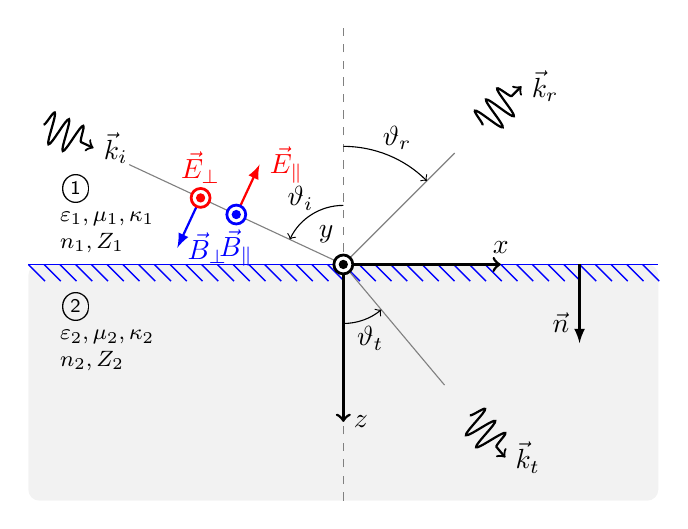
\begin{tikzpicture}[media/.style={font={\footnotesize\sffamily}},wave/.style={decorate,decoration={snake,post length=1.4mm,amplitude=2mm,segment length=2mm},thick},
    interface/.style={
        % The border decoration is a path replacing decorator. 
        % For the interface style we want to draw the original path.
        % The postaction option is therefore used to ensure that the
        % border decoration is drawn *after* the original path.
        postaction={draw,decorate,decoration={border,angle=-45,
                    amplitude=0.3cm,segment length=2mm}}},
    ]
    % Round rectangle
    \fill[gray!10,rounded corners] (-4,-3) rectangle (4,0);
    % Interface
    \draw[blue,line width=.5pt,interface](-4,0)--(4,0);
    % Vertical dashed line
    \draw[dashed,gray](0,-3)--(0,3);
    % Coordinates system
    \draw(0,0.15)node[anchor=south east]{$y$};
    \draw[<->,line width=1pt] (2,0) node[above]{$x$}-|(0,-2) node[right]{$z$};
    % Incidence
    \draw[->,wave]
         (155:4.2cm)--(155:3.5cm)node[right]{$\vec{k}_i$};
    \draw[gray](0:0cm)--(155:3cm);
    \path (0,0)++(123:1cm)node{$\vartheta_i$};
    \draw[->](0,0.75)arc(90:155:.75cm);
    % EField
    \draw[red, -latex,thick](155:1.5)--+(65:0.7)node[right]{$\vec{E}_\parallel$};
    \filldraw[fill=white,draw=blue,line width=1pt](155:1.5)circle(.12cm) node[blue,below,yshift=-1.5]{$\vec{B}_\parallel$}; 
    \filldraw[fill=blue,draw=blue,line width=1pt](155:1.5)circle(.04cm); 

    \draw[blue, -latex,thick](155:2)--+(245:0.7)node[right]{$\vec{B}_\perp$};
    \filldraw[fill=white,draw=red,line width=1pt](155:2)circle(.12cm) node[red,above,yshift=1.5]{$\vec{E}_\perp$}; 
    \filldraw[fill=red,draw=red,line width=1pt](155:2)circle(.04cm); 

    
    % Transmission
    \draw[->,wave]
         (-50:2.5cm)--(-50:3.2cm)node[right]{$\vec{k}_t$};
    \draw[gray](0:0cm)--(-50:2cm);
    \path (0,0)++(-70:1cm)node{$\vartheta_t$};
    \draw[->] (0,-0.75) arc (-90:-50:.75cm);
    % Reflection
    \draw[->,wave]
         (45:2.5cm)--(45:3.2cm)node[right]{$\vec{k}_r$};
    \path (0,0)++(67:1.75cm) node{$\vartheta_r$};
    \draw[gray](0:0cm)--(45:2cm);
   \draw[->] (0,1.5)arc(90:45:1.5cm);
    % Media names
    \path[media] (-3,.6)  node[align=left]{{\larger\textcircled{\smaller[2]1}}\\ $\varepsilon_1,\mu_1,\kappa_1$\\ $n_1, Z_1$}
                 (-3,-.9) node[align=left]{{\larger\textcircled{\smaller[2]2}}\\ $\varepsilon_2,\mu_2,\kappa_2$\\ $n_2, Z_2$};

    % $y$ axis
    \filldraw[fill=white,line width=1pt](0,0)circle(.12cm); 
    \filldraw[fill=black,line width=1pt](0,0)circle(.04cm); 
    % \draw[line width=.6pt] (0,0)
    %                       +(-135:.12cm) -- +(45:.12cm)
    %                       +(-45:.12cm) -- +(135:.12cm);

    \draw[thick,-latex] (3,0) -- (3,-1) node[anchor=south east]{$\vec{n}$};                      
\end{tikzpicture}}
\end{column}
\end{columns}
  \begin{itemize}[<+->]
  \item \alert{Linear polarisierte ebene Welle} am Übergang zweier Medien (hom., isotrop, linear)
  \item Wellenvektor der einfallenden Welle \(\Wellenzahl[v]_i\) und Normalenvektor der Grenzfläche \(\vec{n}\) spannen die \alert{Einfallsebene} auf. OBdA: \(\vec{n} = \einheitsvek{z}\)
\item Indizes: i - inzident, r - reflektiert, t - transmittiert
  \item Zwei Fälle: (1) \(\perp \to \EFeld[v]_i \perp\) zur Einfallsebene (\alert{senkrechte Polarisation}, \enquote{horizontal})\\
    \phantom{Zwei Fälle: }(2) \(\parallel \to \EFeld[v]_i\) in der Einfallsebene (\alert{parallele Polarisation}, \enquote{vertikal})
    \item Zunächst unbekannt: (1) \(\omega_i=\omega_r=\omega_t\)? (2) \(\varphi_r=\varphi_t=0\)? (3) \(\vartheta_i = \vartheta_r\)? 
  \end{itemize}
\end{frame}

\begin{frame}
  \frametitle{Charakterisierung der Wellen}
  \begin{itemize}[<+->]
  \item Wir gehen von harmonischer Zeitabhängigkeit aus:
    \begin{align*}
      \EFeld[uv]_i(\Ortsr[v], t) &= \EFeld[uv]_{0i} \euler^{\komplex(\omega_i t - \Wellenzahl[v]_i \cdot \Ortsr[v])} & \BFeld[uv]_i(\Ortsr[v], t) &= \frac{1}{\omega_i} \left(\Wellenzahl[v]_i \times \EFeld[uv]_i(\Ortsr[v], t)\right)\\
      \EFeld[uv]_r(\Ortsr[v], t) &= \EFeld[uv]_{0r} \euler^{\komplex(\omega_r t - \Wellenzahl[v]_r \cdot \Ortsr[v])} & \BFeld[uv]_r(\Ortsr[v], t) &= \frac{1}{\omega_r} \left(\Wellenzahl[v]_r \times \EFeld[uv]_r(\Ortsr[v], t)\right)\\
      \EFeld[uv]_t(\Ortsr[v], t) &= \EFeld[uv]_{0t} \euler^{\komplex(\omega_t t - \Wellenzahl[v]_t \cdot \Ortsr[v])} & \BFeld[uv]_t(\Ortsr[v], t) &= \frac{1}{\omega_t} \left(\Wellenzahl[v]_t \times \EFeld[uv]_t(\Ortsr[v], t)\right)
    \end{align*}
  \item Allgemeine Beziehung zwischen elektrischen und magnetischen Feldern bei ebene Wellen
    \begin{align*}
      \BFeld[uv] &= \frac{1}{\omega} \left(\Wellenzahl[v] \times \EFeld[uv]\right) = \frac{\Wellenzahl}{\omega} \left(\einheitsvek{k} \times \EFeld[uv]\right) = \frac{1}{\Geschwindigkeit_p} \left(\einheitsvek{k} \times \EFeld[uv]\right) = \sqrt{\varepsilon\mu} \left(\einheitsvek{k} \times \EFeld[uv]\right)\\
      \HFeld[uv] = \frac{1}{\mu}\BFeld[uv] &= \frac{1}{\mu}\sqrt{\varepsilon\mu} \left(\einheitsvek{k} \times \EFeld[uv]\right) = \sqrt{\frac{\varepsilon}{\mu}} \left(\einheitsvek{k} \times \EFeld[uv]\right) = \frac{1}{Z} \left(\einheitsvek{k} \times \EFeld[uv]\right)\\
      \EFeld[uv] &= -Z \left(\einheitsvek{k} \times \HFeld[uv]\right)
      \end{align*}
  \end{itemize}
\end{frame}


\begin{frame}
  \frametitle{Kreisfrequenzen \(\omega_i\), \(\omega_r\) und \(\omega_t\)}
  \begin{itemize}[<+->]
  \item Abschnitt \enquote{Verhalten an Grenzflächen}: Für Normalenvektor \(\vec{n}\) \alert{von {\larger\textcircled{\smaller[2]1}} nach {\larger\textcircled{\smaller[2]2}}}:
    \begin{align*}
      \vec{n} \times \left(\EFeld[v]_2 - \EFeld[v]_1 \right) &=\vec{0} &\text{Tangentialkomponente von \(\EFeld[v]\) stetig}\\
      \vec{n} \cdot \left(\DFeld[v]_2 - \DFeld[v]_1 \right) &=\laddichte{F} &\text{Normalkomponente von \(\DFeld[v]\) unstetig}\\
      \vec{n} \times \left(\HFeld[v]_2 - \HFeld[v]_1 \right) &=\StromDichte[v]_{A} &\text{Tangentialkomponente von \(\HFeld[v]\) unstetig}\\
      \vec{n} \cdot \left(\BFeld[v]_2 - \BFeld[v]_1 \right) &=0 &\text{Normalkomponente von \(\BFeld[v]\) stetig}
    \end{align*}
  \item Betrachte Tangentialkomponente von \(\EFeld[v]\). Für \(z=0\) muss gelten:
    \begin{equation*}
      \vec{n} \times \left( \EFeld[uv]_{0t} \euler^{\komplex(\omega_t t - \Wellenzahl[v]_t \cdot \Ortsr[v])} -\left( \EFeld[uv]_{0i} \euler^{\komplex(\omega_i t - \Wellenzahl[v]_i \cdot \Ortsr[v])} + \EFeld[uv]_{0r} \euler^{\komplex(\omega_r t - \Wellenzahl[v]_r \cdot \Ortsr[v])}\right)\right) \stackrel{!}{=} \vec{0}
    \end{equation*}
  \item Für \alert{beliebige Zeitpunkte \(t \ne 0\) und \(\Ortsr[v] = \vec{0}\)} kann dies nur erfüllt werden, wenn gilt
    \begin{equation*}
      \euler^{\komplex\omega_i t} = \euler^{\komplex\omega_r t} =\euler^{\komplex\omega_t t} \Rightarrow \boxed{\omega_i =\omega_r = \omega_t} \quad \to\text{ Keine Änderung der Frequenz!}
      \end{equation*}
  \end{itemize}
\end{frame}

\begin{frame}
  \frametitle{Wellenvektoren \(\Wellenzahl[v]_r\) und \(\Wellenzahl[v]_t\) in Einfallsebene}
  \begin{itemize}[<+->]
  \item Im gewählten Koordinatensystem gilt
    \begin{align*}
      \Wellenzahl[v]_i &= \Wellenzahl_i \left( \sin\vartheta_i\einheitsvek{x} + \cos\vartheta_i\einheitsvek{z} \right)\\
      \Wellenzahl[v]_r &= \Wellenzahl_r \left( \cos\varphi_r\sin\vartheta_r\einheitsvek{x} + \sin\varphi_r\sin\vartheta_r\einheitsvek{y}  - \cos\vartheta_r\einheitsvek{z}\right) \\
      \Wellenzahl[v]_t &= \Wellenzahl_t \left( \cos\varphi_t\sin\vartheta_t\einheitsvek{x} + \sin\varphi_t\sin\vartheta_t\einheitsvek{y}  + \cos\vartheta_t\einheitsvek{z}\right) 
    \end{align*}
    \item Betrachte Punkt auf der Grenzfläche (\(z=0\)): \(\Ortsr[v] = x\einheitsvek{x} + y\einheitsvek{y} \)
    \begin{align*}
      \Wellenzahl[v]_i\cdot\Ortsr[v] &= \Wellenzahl_i x\sin\vartheta_i \\
      \Wellenzahl[v]_r \cdot\Ortsr[v]&= \Wellenzahl_r \left( x\cos\varphi_r\sin\vartheta_r + y\sin\varphi_r\sin\vartheta_r \right) \\
      \Wellenzahl[v]_t \cdot\Ortsr[v]&= \Wellenzahl_t \left( x\cos\varphi_t\sin\vartheta_t + y\sin\varphi_t\sin\vartheta_t \right) 
    \end{align*}
  \item Für \(t=0\) muss für \(x\)- und \(y\)-Komponente gelten (\(\euler^{-\komplex\Wellenzahl[v]_i\cdot\Ortsr[v]} = \euler^{-\komplex\Wellenzahl[v]_r\cdot\Ortsr[v]} = \euler^{-\komplex\Wellenzahl[v]_t\cdot\Ortsr[v]}\)):
    \begin{equation*}
      \text{x: }\Wellenzahl_i\sin\vartheta_i = \Wellenzahl_r\cos\varphi_r\sin\vartheta_r =\Wellenzahl_t\cos\varphi_t\sin\vartheta_t \quad \text{y: }0=\Wellenzahl_r\sin\varphi_r\sin\vartheta_r = \Wellenzahl_t\sin\varphi_t\sin\vartheta_t
    \end{equation*}
  \item Aus der \(y\)-Komponente folgt für \(\vartheta_r\ne 0\) und \(\vartheta_t\ne 0\): \(\boxed{\varphi_r=\varphi_t=0}\) (\alert{r und t in EFE})
  \end{itemize}
\end{frame}

\begin{frame}
  \frametitle{Reflexions- und Brechungsgesetz}
  \begin{itemize}[<+->]
  \item Die Bedingung für die \(x\)-Komponente vereinfacht sich damit zu
    \begin{equation*}
      \Wellenzahl_i\sin\vartheta_i = \Wellenzahl_r\sin\vartheta_r =\Wellenzahl_t\sin\vartheta_t
    \end{equation*}
  \item Die Beträge der Wellenvektoren sind durch die Materialien bestimmt:
    \begin{align*}
      \Wellenzahl_i = \Wellenzahl_r &= \frac{2\pi}{\lambda_1} = \frac{\omega}{\Geschwindigkeit_{c_1}} = \omega\sqrt{\varepsilon_1\mu_1} = \frac{\omega}{\lichtgeschw}\sqrt{\varepsilon_{r_1}\mu_{r_1}} = \frac{\omega}{\lichtgeschw} n_1 = k_1\\ 
      \Wellenzahl_t &= \frac{2\pi}{\lambda_2} = \frac{\omega}{\Geschwindigkeit_{c_2}} = \omega\sqrt{\varepsilon_2\mu_2} = \frac{\omega}{\lichtgeschw}\sqrt{\varepsilon_{r_2}\mu_{r_2}} = \frac{\omega}{\lichtgeschw} n_2 = k_2
    \end{align*}
  \item Einsetzen in die obige Gleichung ergibt
    \begin{enumerate}[<+->]
    \item Reflexionsgesetz: \(\boxed{\vartheta_i=\vartheta_r}=\vartheta_1\)
      \item Brechungsgesetz nach Snellius: \(\boxed{ n_1\sin\vartheta_1 = n_2\sin\vartheta_2}\) mit \(\vartheta_2=\vartheta_t\)
      \end{enumerate}
      \item Frage nun: Wie stark ist Reflexion bzw. Transmission?
  \end{itemize}
\end{frame}



\begin{frame}
  \frametitle{Reflexions- und Transmissionskoeffizienten}

  \begin{columns}
    \begin{column}{.5\textwidth}
  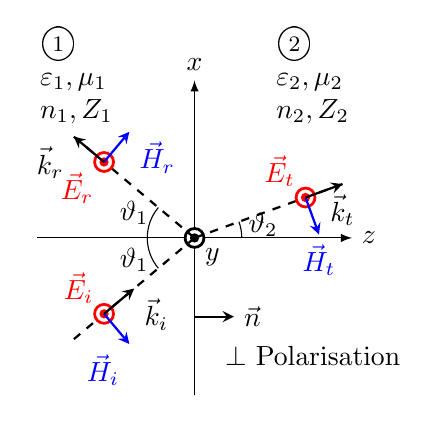
\begin{tikzpicture}
    \draw[-latex, thin] (-2,0) -- (2,0) node[anchor=west] {$z$};
    \draw[-latex, thin] (0,-2) -- (0,2) node[anchor=south] {$x$};
    \filldraw[fill=white,line width=1pt](0,0)circle(.12cm) node[anchor=north west]{$y$}; 
    \filldraw[fill=black,line width=1pt](0,0)circle(.04cm);
\path (-1.5,2)  node[align=left]{{\larger\textcircled{\smaller[2]1}}\\ $\varepsilon_1,\mu_1$\\ $n_1, Z_1$}
(1.5,2) node[align=left]{{\larger\textcircled{\smaller[2]2}}\\ $\varepsilon_2,\mu_2$\\ $n_2, Z_2$};
\draw[dashed, thick] (0,0) -- +(20:2); 
\draw[dashed, thick] (220:2) -- (0,0); 
\draw[dashed, thick] (0,0) -- (140:2);
\draw[thin] (0.6,0) arc (0:20:0.6) node[right,yshift=-1]{$\vartheta_2$}; 
\draw[thin] (-0.6,0) arc (180:220:0.6) node[left,yshift=3]{$\vartheta_1$}; 
\draw[thin] (-0.6,0) arc (180:140:0.6) node[left,yshift=-2]{$\vartheta_1$};

\filldraw[fill=white,line width=1pt, draw=red](140:1.5)circle(.12cm) node[red, anchor=north east]{$\vec{E}_r$};
\filldraw[fill=red,line width=1pt, draw=red](140:1.5)circle(.04cm);
\draw[blue,-stealth, thick] (140:1.5) -- +(50:0.5) node[blue, anchor=north west]{$\vec{H}_r$}; 
\draw[black,-stealth, thick] (140:1.5) -- +(140:0.5) node[anchor=north east]{$\vec{k}_r$}; 


\filldraw[fill=white,line width=1pt, draw=red](220:1.5)circle(.12cm) node[red, anchor=south east]{$\vec{E}_i$};
\filldraw[fill=red,line width=1pt, draw=red](220:1.5)circle(.04cm);
\draw[blue,-stealth, thick] (220:1.5) -- +(310:0.5) node[blue, anchor=north east]{$\vec{H}_i$}; 
\draw[black,-stealth, thick] (220:1.5) -- +(220:-0.5) node[anchor=north west]{$\vec{k}_i$}; 

\filldraw[fill=white,line width=1pt, draw=red](20:1.5)circle(.12cm) node[red, anchor=south east]{$\vec{E}_t$};
\filldraw[fill=red,line width=1pt, draw=red](20:1.5)circle(.04cm);
\draw[blue,-stealth, thick] (20:1.5) -- +(-70:0.5) node[blue, anchor=north]{$\vec{H}_t$}; 
\draw[black,-stealth, thick] (20:1.5) -- +(20:0.5) node[anchor=north]{$\vec{k}_t$};
\draw (1.5,-1.5) node{$\perp$ Polarisation};
\draw[-stealth,thick] (0,-1) -- (0.5,-1) node[anchor=west]{$\vec{n}$}; 
\end{tikzpicture}
\end{column}
\begin{column}{.5\textwidth}
  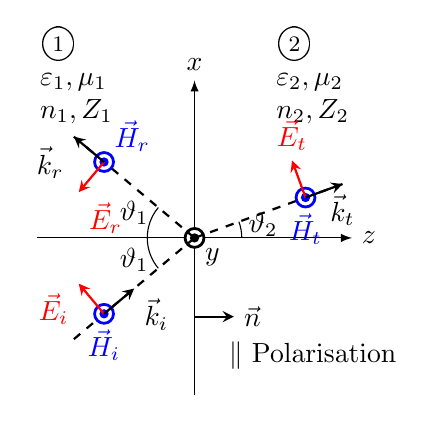
\begin{tikzpicture}
    \draw[-latex, thin] (-2,0) -- (2,0) node[anchor=west] {$z$};
    \draw[-latex, thin] (0,-2) -- (0,2) node[anchor=south] {$x$};
    \filldraw[fill=white,line width=1pt](0,0)circle(.12cm) node[anchor=north west]{$y$}; 
    \filldraw[fill=black,line width=1pt](0,0)circle(.04cm);
\path (-1.5,2)  node[align=left]{{\larger\textcircled{\smaller[2]1}}\\ $\varepsilon_1,\mu_1$\\ $n_1, Z_1$}
(1.5,2) node[align=left]{{\larger\textcircled{\smaller[2]2}}\\ $\varepsilon_2,\mu_2$\\ $n_2, Z_2$};
\draw[dashed, thick] (0,0) -- +(20:2); 
\draw[dashed, thick] (220:2) -- (0,0); 
\draw[dashed, thick] (0,0) -- (140:2);
\draw[thin] (0.6,0) arc (0:20:0.6) node[right,yshift=-1]{$\vartheta_2$}; 
\draw[thin] (-0.6,0) arc (180:220:0.6) node[left,yshift=3]{$\vartheta_1$}; 
\draw[thin] (-0.6,0) arc (180:140:0.6) node[left,yshift=-2]{$\vartheta_1$};

\filldraw[fill=white,line width=1pt, draw=blue](140:1.5)circle(.12cm) node[blue, anchor=south west]{$\vec{H}_r$};
\filldraw[fill=blue,line width=1pt, draw=blue](140:1.5)circle(.04cm);
%\draw[line width=.6pt] (0,0) +(-135:.12cm) -- +(45:.12cm) +(-45:.12cm) -- +(135:.12cm); 
\draw[red,-stealth, thick] (140:1.5) -- +(230:0.5) node[red, anchor=north west]{$\vec{E}_r$}; 
\draw[black,-stealth, thick] (140:1.5) -- +(140:0.5) node[anchor=north east]{$\vec{k}_r$}; 


\filldraw[fill=white,line width=1pt, draw=blue](220:1.5)circle(.12cm) node[blue, anchor=north,yshift=-2]{$\vec{H}_i$};
\filldraw[fill=blue,line width=1pt, draw=blue](220:1.5)circle(.04cm);
%\draw[blue, line width=.6pt] (220:1.5) +(-135:.12cm) -- +(45:.12cm) +(-45:.12cm) -- +(135:.12cm); 
\draw[red,-stealth, thick] (220:1.5) -- +(130:0.5) node[anchor=north east]{$\vec{E}_i$}; 
\draw[black,-stealth, thick] (220:1.5) -- +(220:-0.5) node[anchor=north west]{$\vec{k}_i$}; 

\filldraw[fill=white,line width=1pt, draw=blue](20:1.5)circle(.12cm) node[blue, anchor=north,yshift=-2]{$\vec{H}_t$};
\filldraw[fill=blue,line width=1pt, draw=blue](20:1.5)circle(.04cm);
%\draw[line width=.6pt] (0,0) +(-135:.12cm) -- +(45:.12cm) +(-45:.12cm) -- +(135:.12cm); 
\draw[red,-stealth, thick] (20:1.5) -- +(110:0.5) node[red, anchor=south]{$\vec{E}_t$}; 
\draw[black,-stealth, thick] (20:1.5) -- +(20:0.5) node[anchor=north]{$\vec{k}_t$};
\draw (1.5,-1.5) node{$\parallel$ Polarisation};
\draw[-stealth,thick] (0,-1) -- (0.5,-1) node[anchor=west]{$\vec{n}$}; 
\end{tikzpicture}
\end{column}
\end{columns}
    \begin{align*}
      \vec{n} \times \left(\EFeld[v]_2 - \EFeld[v]_1 \right) &=\vec{0} &\text{Tangentialkomponente von \(\EFeld[v]\) stetig}\\
      \vec{n} \cdot \left(\DFeld[v]_2 - \DFeld[v]_1 \right) &=\laddichte{F} &\text{Normalkomponente von \(\DFeld[v]\) unstetig}\\
      \vec{n} \times \left(\HFeld[v]_2 - \HFeld[v]_1 \right) &=\StromDichte[v]_{A} &\text{Tangentialkomponente von \(\HFeld[v]\) unstetig}\\
      \vec{n} \cdot \left(\BFeld[v]_2 - \BFeld[v]_1 \right) &=0 &\text{Normalkomponente von \(\BFeld[v]\) stetig}
    \end{align*}

\end{frame}

\begin{frame}
  \frametitle{Reflexions- und Transmissionskoeffizienten (\(\perp\))}

  \begin{columns}
    \begin{column}{.3\textwidth}
      \resizebox{\columnwidth}{!}{%
  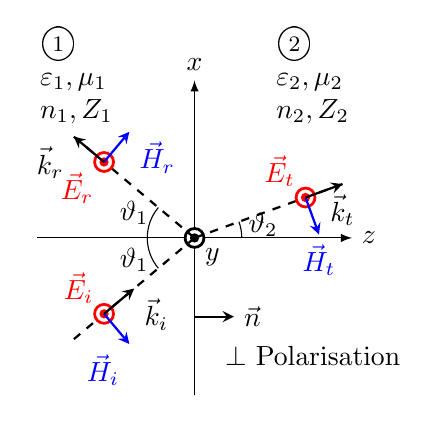
\begin{tikzpicture}
    \draw[-latex, thin] (-2,0) -- (2,0) node[anchor=west] {$z$};
    \draw[-latex, thin] (0,-2) -- (0,2) node[anchor=south] {$x$};
    \filldraw[fill=white,line width=1pt](0,0)circle(.12cm) node[anchor=north west]{$y$}; 
    \filldraw[fill=black,line width=1pt](0,0)circle(.04cm);
\path (-1.5,2)  node[align=left]{{\larger\textcircled{\smaller[2]1}}\\ $\varepsilon_1,\mu_1$\\ $n_1, Z_1$}
(1.5,2) node[align=left]{{\larger\textcircled{\smaller[2]2}}\\ $\varepsilon_2,\mu_2$\\ $n_2, Z_2$};
\draw[dashed, thick] (0,0) -- +(20:2); 
\draw[dashed, thick] (220:2) -- (0,0); 
\draw[dashed, thick] (0,0) -- (140:2);
\draw[thin] (0.6,0) arc (0:20:0.6) node[right,yshift=-1]{$\vartheta_2$}; 
\draw[thin] (-0.6,0) arc (180:220:0.6) node[left,yshift=3]{$\vartheta_1$}; 
\draw[thin] (-0.6,0) arc (180:140:0.6) node[left,yshift=-2]{$\vartheta_1$};

\filldraw[fill=white,line width=1pt, draw=red](140:1.5)circle(.12cm) node[red, anchor=north east]{$\vec{E}_r$};
\filldraw[fill=red,line width=1pt, draw=red](140:1.5)circle(.04cm);
\draw[blue,-stealth, thick] (140:1.5) -- +(50:0.5) node[blue, anchor=north west]{$\vec{H}_r$}; 
\draw[black,-stealth, thick] (140:1.5) -- +(140:0.5) node[anchor=north east]{$\vec{k}_r$}; 


\filldraw[fill=white,line width=1pt, draw=red](220:1.5)circle(.12cm) node[red, anchor=south east]{$\vec{E}_i$};
\filldraw[fill=red,line width=1pt, draw=red](220:1.5)circle(.04cm);
\draw[blue,-stealth, thick] (220:1.5) -- +(310:0.5) node[blue, anchor=north east]{$\vec{H}_i$}; 
\draw[black,-stealth, thick] (220:1.5) -- +(220:-0.5) node[anchor=north west]{$\vec{k}_i$}; 

\filldraw[fill=white,line width=1pt, draw=red](20:1.5)circle(.12cm) node[red, anchor=south east]{$\vec{E}_t$};
\filldraw[fill=red,line width=1pt, draw=red](20:1.5)circle(.04cm);
\draw[blue,-stealth, thick] (20:1.5) -- +(-70:0.5) node[blue, anchor=north]{$\vec{H}_t$}; 
\draw[black,-stealth, thick] (20:1.5) -- +(20:0.5) node[anchor=north]{$\vec{k}_t$};
\draw (1.5,-1.5) node{$\perp$ Polarisation};
\draw[-stealth,thick] (0,-1) -- (0.5,-1) node[anchor=west]{$\vec{n}$}; 
\end{tikzpicture}}
\end{column}
\begin{column}{.7\textwidth}
  \begin{itemize}[<+->]
  \item Betrachtung \(\EFeld[v]\) (in y-Richtung)
  \item k-Richtungen
    \begin{align*}
      \einheitsvek{k_i} &= \sin\vartheta_1\einheitsvek{x} + \cos\vartheta_1\einheitsvek{z} \\
      \einheitsvek{k_r} &= \sin\vartheta_1\einheitsvek{x} - \cos\vartheta_1\einheitsvek{z} \\
      \einheitsvek{k_t} &= \sin\vartheta_2\einheitsvek{x} + \cos\vartheta_2\einheitsvek{z} 
    \end{align*}
  \item Ortsvektor bei \(z=0
    \): \(\Ortsr[v] = x\einheitsvek{x} + y \einheitsvek{y}\)
    \end{itemize}
\end{column}
\end{columns}

\begin{itemize}[<+->]
\item Stetigkeit der Tangentialkomponente von \(\EFeld[v]\)
    \begin{align*}
      \einheitsvek{z} \times \left(\EFeld[u]_{0i} \einheitsvek{y}\euler^{-\komplex \Wellenzahl_i x \sin\vartheta_1} + \EFeld[u]_{0r} \einheitsvek{y}\euler^{-\komplex \Wellenzahl_r x \sin\vartheta_1}   \right) &= \einheitsvek{z} \times \EFeld[u]_{0t} \einheitsvek{y}\euler^{-\komplex \Wellenzahl_t x \sin\vartheta_2} \; ; \; \einheitsvek{z} \times \einheitsvek{y} = -\einheitsvek{x} \\
      -\einheitsvek{x}  \left(\EFeld[u]_{0i} \euler^{-\komplex \Wellenzahl_i x \sin\vartheta_1} + \EFeld[u]_{0r}\euler^{-\komplex \Wellenzahl_r x \sin\vartheta_1}   \right) &= -\einheitsvek{x}  \EFeld[u]_{0t} \euler^{-\komplex \Wellenzahl_t x \sin\vartheta_2} 
    \end{align*}
  \item Für \(x=0\) folgt:
    \begin{equation*}
      \boxed{ \EFeld[u]_{0i} + \EFeld[u]_{0r}= \EFeld[u]_{0t}}
      \end{equation*}
    \end{itemize}
\end{frame}


\begin{frame}
  \frametitle{Reflexions- und Transmissionskoeffizienten (\(\perp\))}

  \begin{columns}
    \begin{column}{.3\textwidth}
      \resizebox{\columnwidth}{!}{%
  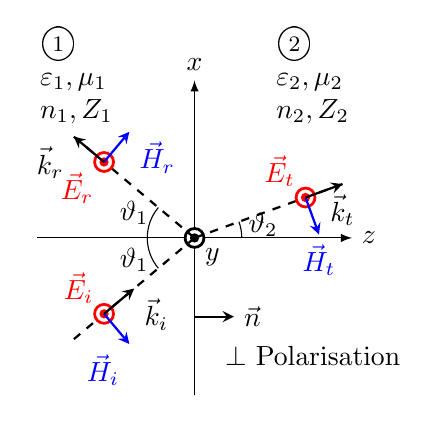
\begin{tikzpicture}
    \draw[-latex, thin] (-2,0) -- (2,0) node[anchor=west] {$z$};
    \draw[-latex, thin] (0,-2) -- (0,2) node[anchor=south] {$x$};
    \filldraw[fill=white,line width=1pt](0,0)circle(.12cm) node[anchor=north west]{$y$}; 
    \filldraw[fill=black,line width=1pt](0,0)circle(.04cm);
\path (-1.5,2)  node[align=left]{{\larger\textcircled{\smaller[2]1}}\\ $\varepsilon_1,\mu_1$\\ $n_1, Z_1$}
(1.5,2) node[align=left]{{\larger\textcircled{\smaller[2]2}}\\ $\varepsilon_2,\mu_2$\\ $n_2, Z_2$};
\draw[dashed, thick] (0,0) -- +(20:2); 
\draw[dashed, thick] (220:2) -- (0,0); 
\draw[dashed, thick] (0,0) -- (140:2);
\draw[thin] (0.6,0) arc (0:20:0.6) node[right,yshift=-1]{$\vartheta_2$}; 
\draw[thin] (-0.6,0) arc (180:220:0.6) node[left,yshift=3]{$\vartheta_1$}; 
\draw[thin] (-0.6,0) arc (180:140:0.6) node[left,yshift=-2]{$\vartheta_1$};

\filldraw[fill=white,line width=1pt, draw=red](140:1.5)circle(.12cm) node[red, anchor=north east]{$\vec{E}_r$};
\filldraw[fill=red,line width=1pt, draw=red](140:1.5)circle(.04cm);
\draw[blue,-stealth, thick] (140:1.5) -- +(50:0.5) node[blue, anchor=north west]{$\vec{H}_r$}; 
\draw[black,-stealth, thick] (140:1.5) -- +(140:0.5) node[anchor=north east]{$\vec{k}_r$}; 


\filldraw[fill=white,line width=1pt, draw=red](220:1.5)circle(.12cm) node[red, anchor=south east]{$\vec{E}_i$};
\filldraw[fill=red,line width=1pt, draw=red](220:1.5)circle(.04cm);
\draw[blue,-stealth, thick] (220:1.5) -- +(310:0.5) node[blue, anchor=north east]{$\vec{H}_i$}; 
\draw[black,-stealth, thick] (220:1.5) -- +(220:-0.5) node[anchor=north west]{$\vec{k}_i$}; 

\filldraw[fill=white,line width=1pt, draw=red](20:1.5)circle(.12cm) node[red, anchor=south east]{$\vec{E}_t$};
\filldraw[fill=red,line width=1pt, draw=red](20:1.5)circle(.04cm);
\draw[blue,-stealth, thick] (20:1.5) -- +(-70:0.5) node[blue, anchor=north]{$\vec{H}_t$}; 
\draw[black,-stealth, thick] (20:1.5) -- +(20:0.5) node[anchor=north]{$\vec{k}_t$};
\draw (1.5,-1.5) node{$\perp$ Polarisation};
\draw[-stealth,thick] (0,-1) -- (0.5,-1) node[anchor=west]{$\vec{n}$}; 
\end{tikzpicture}}
\end{column}
\begin{column}{.7\textwidth}
  \begin{itemize}[<+->]
  \item Betrachtung \(\HFeld[v]\)
  \item Oberflächenstromdichte \(\StromDichte[v]_A = \vec{0}\) (vgl. Felddiffusion im Halbraum)
    \begin{align*}
      \einheitsvek{z} \times \left( \HFeld[v]_i + \HFeld[v]_r \right) &= \einheitsvek{z} \times \HFeld[v]_t  \quad \HFeld[v] = \frac{1}{Z} \einheitsvek{k} \times \EFeld[v] \\ 
      \einheitsvek{z} \times \left( \frac{1}{Z_1} \einheitsvek{k_i} \times \EFeld[v]_i + \frac{1}{Z_1} \einheitsvek{k_r} \times \EFeld[v]_r \right) &= \einheitsvek{z} \times \frac{1}{Z_2} \einheitsvek{k_t} \times \EFeld[v]_t  
    \end{align*}
    \end{itemize}
\end{column}
\end{columns}

\begin{itemize}[<+->]
\item Auflösen des doppelten Kreuzproduktes (nutze: \(\einheitsvek{z}\cdot \EFeld[v]_{irt}=0\))
  \begin{align*}
    \frac{1}{Z_1}\left[   - \EFeld[v]_i\left(\einheitsvek{z}\cdot \einheitsvek{k_i}  \right)  - \EFeld[v]_r\left(\einheitsvek{z}\cdot \einheitsvek{k_r}  \right) \right] &= \frac{1}{Z_2}\left[   - \EFeld[v]_t\left(\einheitsvek{z}\cdot \einheitsvek{k_t}  \right)\right]\\
    \frac{1}{Z_1}\left[   - \cos\vartheta_1\EFeld[v]_i  +\cos\vartheta_1 \EFeld[v]_r \right] &= -\frac{1}{Z_2} \cos\vartheta_2 \EFeld[v]_t\\
    \Aboxed{\frac{1}{Z_1}\left[   \cos\vartheta_1\EFeld[u]_{0i}  -\cos\vartheta_1 \EFeld[u]_{0r} \right] &= \frac{1}{Z_2} \cos\vartheta_2 \EFeld[u]_{0t}}
    \end{align*}
    \end{itemize}
\end{frame}


\begin{frame}
  \frametitle{Reflexions- und Transmissionskoeffizienten (\(\perp\))}  
\begin{itemize}[<+->]
\item Zwei Beziehungen gefunden:
  \begin{equation*}
    \EFeld[u]_{0i} + \EFeld[u]_{0r}= \EFeld[u]_{0t} \quad\text{ und }\quad \frac{1}{Z_1}\left[   \cos\vartheta_1\EFeld[u]_{0i}  -\cos\vartheta_1 \EFeld[u]_{0r} \right] = \frac{1}{Z_2} \cos\vartheta_2 \EFeld[u]_{0t}
  \end{equation*}
\item Damit können der \alert{Reflexions-} und der \alert{Transmissionskoeffizient}
  \begin{equation*}
    \underline{r}_\perp = \frac{\EFeld[u]_{0r}}{\EFeld[u]_{0i}} \qquad \underline{t}_\perp = \frac{\EFeld[u]_{0t}}{\EFeld[u]_{0i}} \quad\text{ bestimmt werden.} 
  \end{equation*}
\item Aus der ersten Gleichung ergibt sich
  \begin{equation*}
    \EFeld[u]_{0i} + \EFeld[u]_{0r}= \EFeld[u]_{0t} \Rightarrow  1+ \frac{\EFeld[u]_{0r}}{\EFeld[u]_{0i}}= \frac{\EFeld[u]_{0t}}{\EFeld[u]_{0i}} \Rightarrow \boxed{1+\underline{r}_\perp = \underline{t}_\perp}
\end{equation*}
\item Aus der zweiten Gleichung ergibt sich
  \begin{equation*}
    \frac{1}{Z_1}\left[   \cos\vartheta_1\EFeld[u]_{0i}  -\cos\vartheta_1 \EFeld[u]_{0r} \right] = \frac{1}{Z_2} \cos\vartheta_2 \EFeld[u]_{0t} \Rightarrow  \boxed{Z_2\cos\vartheta_1\left(1-\underline{r}_\perp\right) = Z_1 \cos\vartheta_2\underline{t}_\perp}
\end{equation*}
  \end{itemize}
\end{frame}

\begin{frame}
  \frametitle{Reflexions- und Transmissionskoeffizienten (\(\perp\))}  
\begin{itemize}[<+->]
\item Wir hatten 
  \begin{equation*}
    1+\underline{r}_\perp = \underline{t}_\perp \text{ und } Z_2\cos\vartheta_1\left(1-\underline{r}_\perp\right) = Z_1 \cos\vartheta_2\underline{t}_\perp
  \end{equation*}
  \item Hieraus ergeben sich Reflexions- und Transmissionskoeffizient (\alert{Fresnelsche Beziehungen}) zu
    \begin{align*}
\Aboxed{\underline{r}_\perp &= \frac{Z_2\cos\vartheta_1-Z_1\cos\vartheta_2}{Z_1\cos\vartheta_2+Z_2\cos\vartheta_1}} \\
1+\underline{r}_\perp = \Aboxed{\underline{t}_\perp &= \frac{2 Z_2\cos\vartheta_1}{Z_1\cos\vartheta_2+Z_2\cos\vartheta_1}} 
    \end{align*}
  \item Wichtiger Spezialfall: Übergang Luft-Metall\\
    Luft: \(Z=Z_1\simeq\SI{377}{\ohm}\)\\
    Metall: \({\displaystyle Z=Z_2 = \sqrt{\frac{\mu}{\underline{\varepsilon}}}  = \sqrt{\frac{\mu}{\varepsilon_0\left(\varepsilon_r -\komplex\frac{\kappa}{\varepsilon_0\omega}\right)}} \simeq (1+\komplex)\sqrt{\frac{\mu\omega}{2\kappa}} \to \left|Z_2\right| \ll \SI{377}{\ohm}}\)
    \begin{equation*}
    \Rightarrow \boxed{\underline{r}_\perp \simeq -1 \quad \underline{t}_\perp \simeq 0}
    \end{equation*}
\end{itemize}
\end{frame}

\begin{frame}
  \frametitle{Reflexions- und Transmissionskoeffizienten (\(\parallel\))}  
  \begin{itemize}[<+->]
  \item Die Herleitung von Reflexions- und Transmissionskoeffizienten für \alert{parallele Polarisation} verläuft völlig analog und wird hier nicht wiederholt.
  \item Die Unterschiede in den \alert{Fresnelschen Beziehungen} werden im direkten Vergleich deutlich:
    \begin{align*}
\Aboxed{\underline{r}_\perp &= \frac{Z_2\cos\vartheta_1-Z_1\cos\vartheta_2}{Z_1\cos\vartheta_2+Z_2\cos\vartheta_1}} \\
      1+\underline{r}_\perp =
\Aboxed{\underline{t}_\perp &= \frac{2 Z_2\cos\vartheta_1}{Z_1\cos\vartheta_2+Z_2\cos\vartheta_1}} \\
\Aboxed{\underline{r}_\parallel &= \frac{Z_1\cos\vartheta_1-Z_2\cos\vartheta_2}{Z_2\cos\vartheta_2+Z_1\cos\vartheta_1}} \\
      \frac{Z_2}{Z_1}\left(1+\underline{r}_\parallel\right)=\frac{\cos\vartheta_1}{\cos\vartheta_2}\left(1-\underline{r}_\parallel\right)
= \Aboxed{\underline{t}_\parallel &= \frac{2 Z_2\cos\vartheta_1}{Z_2\cos\vartheta_2+Z_1\cos\vartheta_1}} 
    \end{align*}
\item Für den Übergang Luft-Metall folgt hier (Unterschied folgt sofort aus der Stetigkeitsbedingung für die Tangentialkomponente des E-Feldes \(\to\) Selbstübung):     
    \begin{equation*}
    \Rightarrow \boxed{\underline{r}_\parallel \simeq +1 \quad \underline{t}_\parallel \simeq 0}
    \end{equation*}
\end{itemize}
\end{frame}

\begin{frame}
  \frametitle{Reflexions- und Transmissionskoeffizienten (mit \(n\))}  
  \begin{itemize}[<+->]
  \item Mit \(Z=\sqrt{\nicefrac{\mu}{\varepsilon}}\) und \(n=\sqrt{\varepsilon_r\mu_r}\) folgt \(Z = \nicefrac{\mu\lichtgeschw}{n}\), so dass für die Reflexions- und Transmissionskoeffizienten folgt
\begin{align*}
\Aboxed{\underline{r}_\perp &= \frac{n_1\cos\vartheta_1-\frac{\mu_1}{\mu_2} n_2\cos\vartheta_2}{n_1\cos\vartheta_1+\frac{\mu_1}{\mu_2} n_2\cos\vartheta_2}} & \Aboxed{\underline{t}_\perp &= \frac{2 n_1\cos\vartheta_1}{n_1\cos\vartheta_1+\frac{\mu_1}{\mu_2} n_2\cos\vartheta_2}} \\
\Aboxed{\underline{r}_\parallel &= \frac{-n_1\cos\vartheta_2+\frac{\mu_1}{\mu_2} n_2\cos\vartheta_1}{n_1\cos\vartheta_2+\frac{\mu_1}{\mu_2} n_2\cos\vartheta_1}} &\Aboxed{\underline{t}_\parallel &= \frac{2 n_1\cos\vartheta_1}{n_1\cos\vartheta_2+\frac{\mu_1}{\mu_2} n_2\cos\vartheta_1}} 
    \end{align*}
  \item Wichtiger Spezialfall: \alert{\(\mu_1 = \mu_2\)}, z.B. beide unmagnetisch
\begin{align*}
\Aboxed{\underline{r}_\perp &= \frac{n_1\cos\vartheta_1- n_2\cos\vartheta_2}{n_1\cos\vartheta_1+ n_2\cos\vartheta_2}} & \Aboxed{\underline{t}_\perp &= \frac{2 n_1\cos\vartheta_1}{n_1\cos\vartheta_1+ n_2\cos\vartheta_2}} \\
\Aboxed{\underline{r}_\parallel &= \frac{-n_1\cos\vartheta_2+n_2\cos\vartheta_1}{n_1\cos\vartheta_2+ n_2\cos\vartheta_1}} &\Aboxed{\underline{t}_\parallel &= \frac{2 n_1\cos\vartheta_1}{n_1\cos\vartheta_2+ n_2\cos\vartheta_1}} 
    \end{align*}
    
\end{itemize}
\end{frame}


\begin{frame}
  \frametitle{Reflexions- und Transmissionskoeffizienten (\(\vartheta_1,\;\vartheta_2\))}  
  \begin{itemize}[<+->]
  \item Im Falle \alert{\(\mu_1 = \mu_2\)} können die Fresnelschen-Beziehungen mit Hilfe des Brechungsgesetzes \(n_1\sin\vartheta_1=n_2\sin\vartheta_2\) auch nur mit den Winkeln geschrieben werden:
\begin{align*}
  \Aboxed{\underline{r}_\perp &= \frac{\cos\vartheta_1- \frac{\sin\vartheta_1}{\sin\vartheta_2}\cos\vartheta_2}{\cos\vartheta_1+ \frac{\sin\vartheta_1}{\sin\vartheta_2}\cos\vartheta_2} = \frac{\sin\left(\vartheta_2-\vartheta_1\right)}{\sin\left(\vartheta_1+\vartheta_2\right)}}\\
  \Aboxed{\underline{t}_\perp &= \frac{2 \cos\vartheta_1}{\cos\vartheta_1+ \frac{\sin\vartheta_1}{\sin\vartheta_2}\cos\vartheta_2} = \frac{2\sin\vartheta_2\cos\vartheta_1}{\sin\left(\vartheta_1+\vartheta_2\right)}} \\
  \Aboxed{\underline{r}_\parallel &= \frac{-\cos\vartheta_2+ \frac{\sin\vartheta_1}{\sin\vartheta_2}\cos\vartheta_1}{\cos\vartheta_2+ \frac{\sin\vartheta_1}{\sin\vartheta_2}\cos\vartheta_1}=\frac{\tan\left(\vartheta_1-\vartheta_2\right)}{\tan\left(\vartheta_1+\vartheta_2\right)}}\\
  \Aboxed{\underline{t}_\parallel &= \frac{2 \cos\vartheta_1}{\cos\vartheta_2+ \frac{\sin\vartheta_1}{\sin\vartheta_2}\cos\vartheta_1}= \frac{2\sin\vartheta_2\cos\vartheta_1}{\sin\left(\vartheta_1+\vartheta_2\right) \cos\left(\vartheta_1-\vartheta_2\right)}} 
    \end{align*}
\end{itemize}
\end{frame}

\begin{frame}
  \frametitle{Verschwinden der Reflexion -- Brewster-Winkel}  
  \begin{itemize}[<+->]
  \item Aus den Reflexionskoeffizienten können die Bedingungen für das \alert{Verschwinden der Reflexion} abgelesen werden:
\begin{align*}
  \underline{r}_\perp &= \frac{\sin\left(\vartheta_2-\vartheta_1\right)}{\sin\left(\vartheta_1+\vartheta_2\right)} & \underline{r}_\parallel &= \frac{\tan\left(\vartheta_1-\vartheta_2\right)}{\tan\left(\vartheta_1+\vartheta_2\right)}
\end{align*}
\item Fall 1: \(\vartheta_1=\vartheta_2 \to n_1=n_2 \to\) \alert{optische gleiches Material}
\item Fall 2: Nur für \alert{parallele Polarisation} ergibt sich eine weitere Möglichkeit
   \begin{equation*}
     \underline{r}_\parallel = \frac{\tan\left(\vartheta_1-\vartheta_2\right)}{\tan\left(\vartheta_1+\vartheta_2\right)} \to 0 \text{ für } \boxed{\vartheta_1+\vartheta_2 = \frac{\pi}{2}} \Rightarrow \alert{\Wellenzahl[v]_r \perp \Wellenzahl[v]_t}
   \end{equation*}
\item Nach dem Brechungsgesetz von Snellius gilt in diesem Fall:
  \begin{equation*}
    \frac{\sin\vartheta_1}{\sin\vartheta_2} = \frac{\sin\vartheta_1}{\sin\left(\nicefrac{\pi}{2}-\vartheta_1\right)} = \frac{\sin\vartheta_1}{\cos\vartheta_1} = \boxed{\tan\vartheta_1=\frac{n_2}{n_1} } \alert{\text{ Brewsterscher Polarisationswinkel}}
  \end{equation*}
  \item Beliebig pol. Welle \(\to\) Reflexion ist \(\perp\) polarisiert! \(\to\) \alert{Polarisator}
\end{itemize}
\end{frame}

\begin{frame}
  \frametitle{Totalreflexion}
  \begin{itemize}[<+->]
  \item Brechungsgesetz: \(n_1\sin\vartheta_1 = n_2\sin\vartheta_2\)
   \item Übergang zum \alert{optisch dichteren Medium}: \(n_1 < n_2\Rightarrow \vartheta_1 > \vartheta_2\)  
   \item Übergang zum \alert{optisch dünnerem Medium}: \(n_1 > n_2\Rightarrow \vartheta_1 < \vartheta_2\)
       \begin{itemize}[<+->]
       \item In diesem Fall wird bei Vergrößerung von \(\vartheta_1\) irgendwann \(\vartheta_2 = \nicefrac{\pi}{2}\) erreicht.
       \item Es wird dann nichts mehr transmittiert \(\to\) \alert{Totalreflexion}
       \item Der \alert{Grenzwinkel der Totalreflexion} \(\vartheta_{1G}\) ist bestimmt durch
         \begin{equation*}
           \boxed{\sin\vartheta_{1G} = \frac{n_2}{n_1}}
         \end{equation*}
         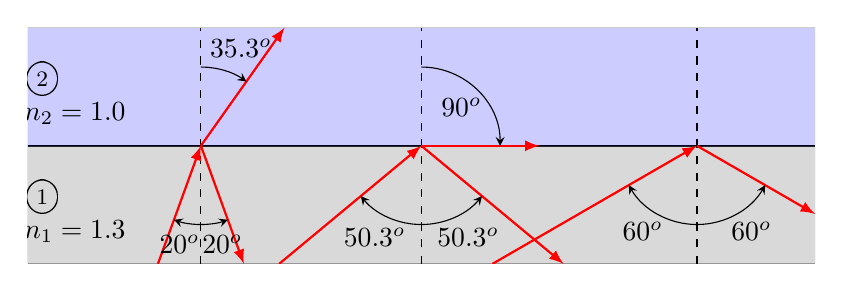
\begin{tikzpicture}
           \clip  (-5,-1.5) rectangle (5,1.5);
           \path [name path=unten] (-5,-1.5) -- (5,-1.5); 
           \path [name path=mitte] (-5,0) -- (5,0); 
           \path [name path=oben] (-5,1.5) -- (5,1.5);
           \path [name path=right] (5,-2) -- (5,2);
           \draw[thick] (-5,0) -- (5,0);
           \draw[fill=gray, opacity=0.3] (-5,-1.5) rectangle (5,0); 
           \draw[fill=blue, opacity=0.2] (-5,0) rectangle (5,1.5); 
\path (-4.4,.6)  node[align=left]{{\larger\textcircled{\smaller[2]2}}\\ $n_2=1.0$}
(-4.4,-.9) node[align=left]{{\larger\textcircled{\smaller[2]1}}\\ $n_1=1.3$};
\draw[thin,dashed] (-2.8,-1.5) -- (-2.8,1.5);
\draw[thin,dashed] (0,-1.5) -- (0,1.5); 
\draw[thin,dashed] (3.5,-1.5) -- (3.5,1.5); 

% 20
\path [name path=ineins] (-2.8,0) -- +(250:4);  % 20
\path [name path=refeins] (-2.8,0) -- +(290:4); % 20
\path [name path=traeins] (-2.8,0) -- +(54.7:4); % 35.3
\draw[name intersections={of=unten and ineins, by=u1}] [red, thick, -latex] (u1) -- (-2.8,0); 
\draw[name intersections={of=unten and refeins, by=u2}] [red, thick, -latex] (-2.8,0) --(u2); 
\draw[name intersections={of=oben and traeins, by=o1}] [red, thick, -latex] (-2.8,0) --(o1);
\draw[thin, -stealth] (-2.8,-1) arc (270:250:1) node[below,xshift=2,yshift=-2]{$20^o$}; 
\draw[thin, -stealth] (-2.8,-1) arc (270:290:1) node[below,xshift=-2,yshift=-2]{$20^o$}; 
\draw[thin, -stealth] (-2.8,1) arc (90:54.7:1) node[above,xshift=-2,yshift=5]{$35.3^o$}; 
% Grenzwinkel = 50.3
\path [name path=inzwei] (0,0) -- +(219.7:4);  % 50.3
\path [name path=refzwei] (0,0) -- +(-39.7:4); % 50.3
%\path [name path=trazwei] (0,0) -- +(0:4); % 90
\draw[name intersections={of=unten and inzwei, by=u3}] [red, thick, -latex] (u3) -- (0,0); 
\draw[name intersections={of=unten and refzwei, by=u4}] [red, thick, -latex] (0,0) -- (u4); 
\draw[red, thick, -latex] (0,0) -- +(0:1.5);
\draw[thin, -stealth] (0,-1) arc (270:219.7:1) node[below,xshift=5,yshift=-8]{$50.3^o$}; 
\draw[thin, -stealth] (0,-1) arc (270:320.3:1) node[below,xshift=-5,yshift=-8]{$50.3^o$}; 
\draw[thin, -stealth] (0,1) arc (90:0:1) node[above,xshift=-14,yshift=7]{$90^o$}; 
% 60
\path [name path=indrei] (3.5,0) -- +(210:4);  % 60
\path [name path=refdrei] (3.5,0) -- +(330:4); % 60
\draw[name intersections={of=unten and indrei, by=u5}] [red, thick, -latex] (u5) -- (3.5,0); 
\draw[name intersections={of=refdrei and right, by=u6}] [red, thick, -latex] (3.5,0) -- (u6); 
\draw[thin, -stealth] (3.5,-1) arc (270:210:1) node[below,xshift=5,yshift=-10]{$60^o$}; 
\draw[thin, -stealth] (3.5,-1) arc (270:330:1) node[below,xshift=-5,yshift=-10]{$60^o$}; 
\end{tikzpicture}
         \item Anwendung: Lichtwellenleiter (Glasfaser), Reflexionsprisma
  \end{itemize}
  \end{itemize}
\ 
\end{frame}

\begin{frame}
  \frametitle{Programme zur Berechnung}
  \begin{itemize}[<+->]
    \item SimPy \(\to\) Physics \(\to\) Optics Module (\url{https://www.sympy.org})
  \item Java Applet der Universität Barcelona: \url{http://www.ub.edu/javaoptics/docs_applets/Doc_PolarEn.html}

    \centering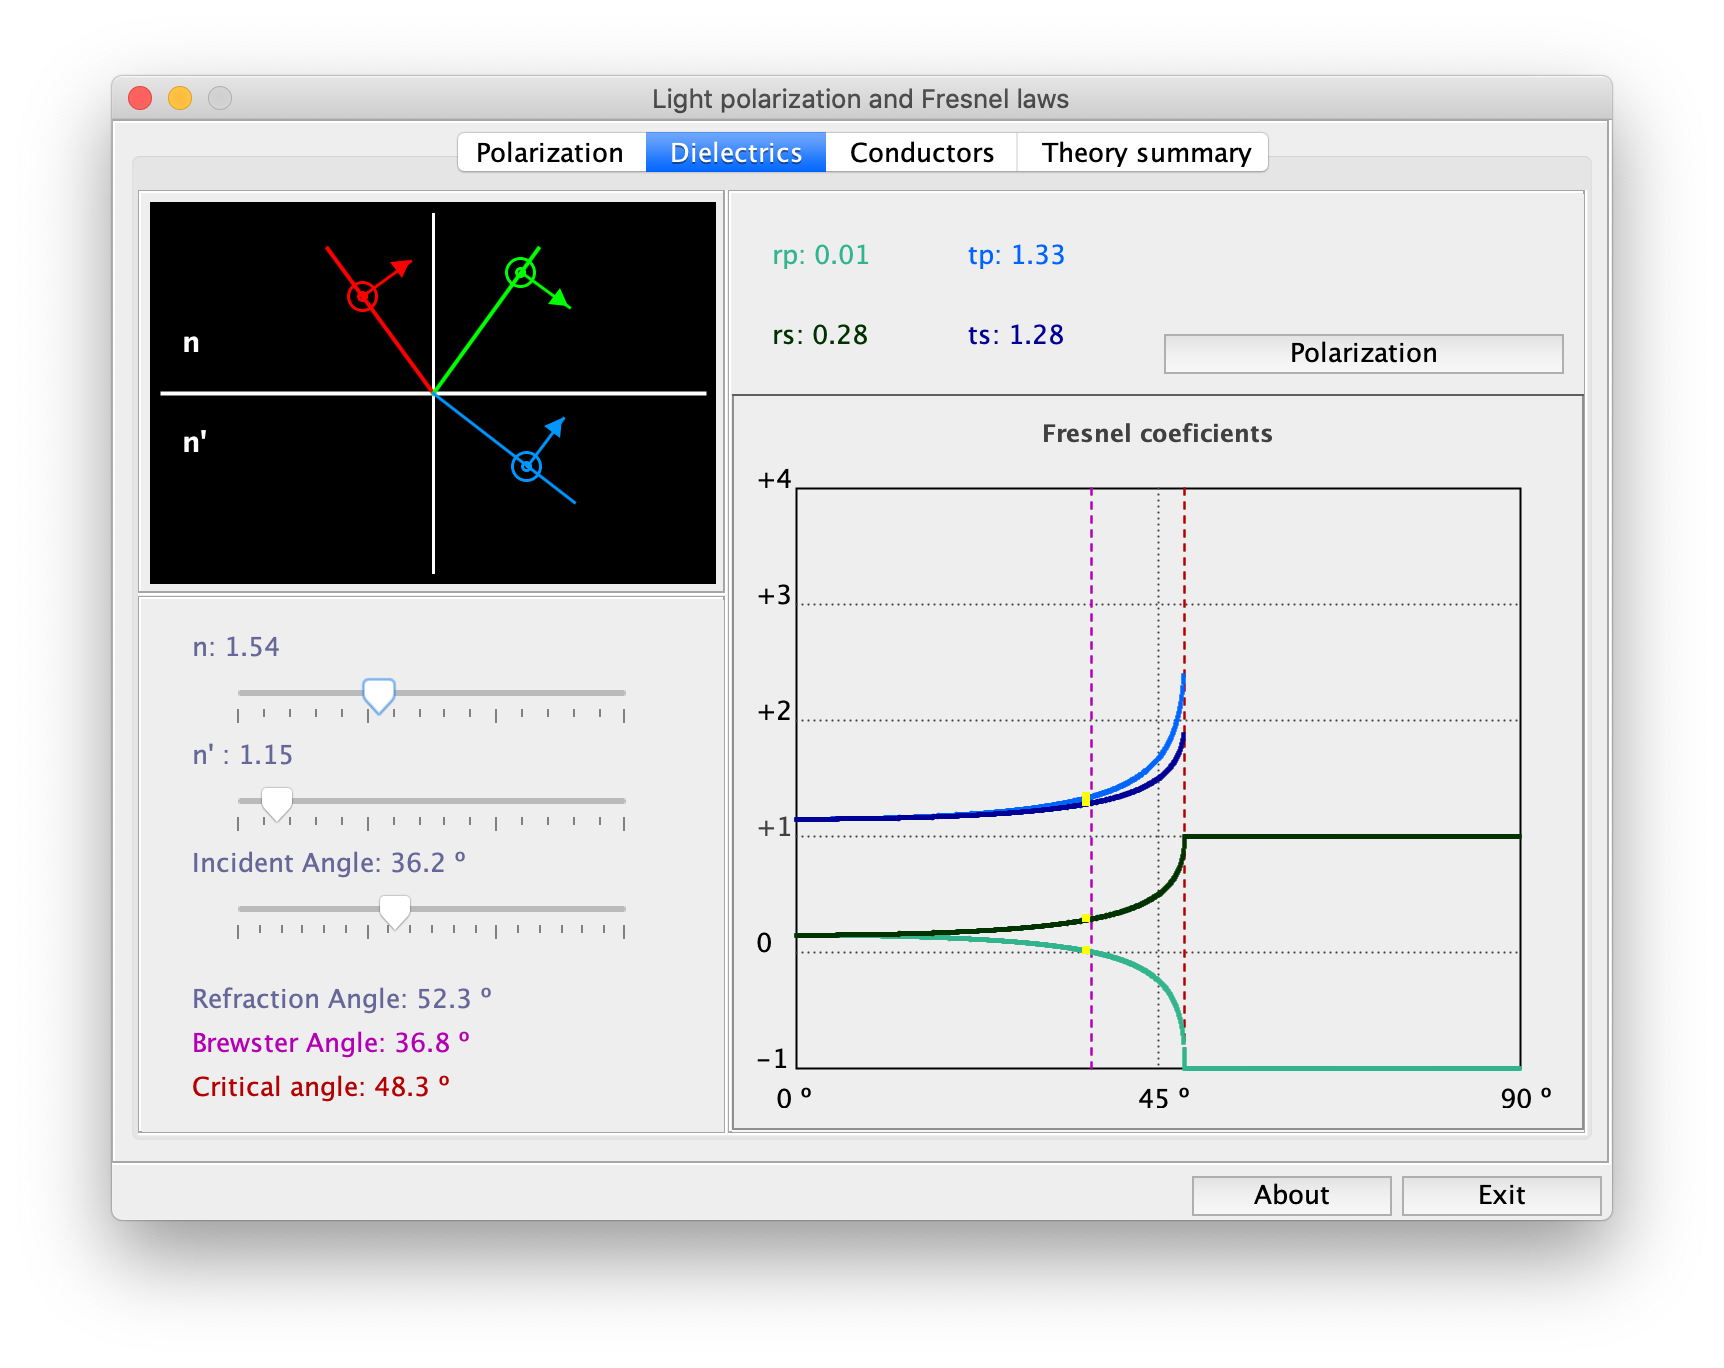
\includegraphics[width=.7\textwidth]{Fresnel-applet}
  \end{itemize}
\end{frame}



\begin{frame}
  \frametitle{Totalreflexion -- Feld im Medium 2}  
  \begin{itemize}[<+->]
       \item Frage: Ist Medium 2 bei Totalreflexion (\(\vartheta_1> \vartheta_{1G}\)) feldfrei? 
  \item \alert{Grenzwinkel der Totalreflexion} beim \alert{Übergang in ein optisch dünneres Medium}:
         \begin{equation*}
           \sin\vartheta_{1G} = \frac{n_2}{n_1} \Rightarrow \frac{n_1}{n_2}\sin\vartheta_{1G} = 1 \Rightarrow \boxed{\frac{n_1}{n_2}\sin\vartheta_{1} > 1 \text{ für } \vartheta_{1}>\vartheta_{1G}}
         \end{equation*}
       \item Wir betrachten \(\Wellenzahl[v]_t\):
         \begin{align*}
           \Wellenzahl[v]_t=\Wellenzahl_2 \einheitsvek{k_t} &= \Wellenzahl_2 \left( \sin\vartheta_2\einheitsvek{x} +   \cos\vartheta_2\einheitsvek{z}\right) \\
                                                        &= \Wellenzahl_2 \left(\frac{n_1}{n_2} \sin\vartheta_1\einheitsvek{x} \pm \sqrt{\left(1-   \sin^2\vartheta_2\right)}\;\einheitsvek{z}\right)\\
                                                        &= \Wellenzahl_2 \left(\frac{n_1}{n_2} \sin\vartheta_1\einheitsvek{x} \pm \sqrt{\left(1-  \left(\frac{n_1}{n_2}\right)^2 \sin^2\vartheta_1\right)}\;\einheitsvek{z}\right)\\
                                                        &= \Wellenzahl_2 \left(\frac{n_1}{n_2} \sin\vartheta_1\einheitsvek{x} \pm \komplex\sqrt{\left( \left(\frac{n_1}{n_2}\right)^2 \sin^2\vartheta_1-1\right)}\;\einheitsvek{z}\right)\\
           &= \beta \einheitsvek{x} \pm \komplex \alpha \einheitsvek{z} 
           \end{align*}
\end{itemize}
\end{frame}

\begin{frame}
  \frametitle{Totalreflexion -- Feld im Medium 2 (\dots)}  
  \begin{itemize}[<+->]
  \item Für das elektrische Feld im Medium 2 ergibt sich mit diesem Wellenvektor und dem Transmissionskoeffizienten \(t\)
    \begin{align*}
      \EFeld[uv]_t &= t \EFeld[u]_{0i} \euler^{\komplex \left(\omega t - \Wellenzahl[v]_t\cdot\Ortsr[v] \right)} \einheitsvek{E_t}\\
                   &= t \EFeld[u]_{0i} \euler^{\pm\alpha z} \euler^{\komplex\left(\omega t - \beta x \right)}\einheitsvek{E_t} \quad \text{\(+\alpha z\) Lösung unphysikalisch} \\
       &= t \EFeld[u]_{0i} \euler^{-\alpha z} \euler^{\komplex\left(\omega t - \beta x \right)}\einheitsvek{E_t} \quad \text{exponentialler Abfall in z; Welle in x}
    \end{align*}
  \item Poyntingscher Vektor:
    \begin{align*}
      \PoyntingVektor[uv] &= \frac{1}{2} \EFeld[uv]_t \times \HFeld[uv]_t^\star = \frac{1}{2 Z_2} \EFeld[uv]_t \times \left(\einheitsvek{k_t}^\star \times \EFeld[uv]_t^\star\right) = \frac{1}{2 Z_2} \left|\EFeld[uv]_t\right|^2 \einheitsvek{k_t}^\star \; ,\; \Wellenzahl[uv]_t = \beta \einheitsvek{x} - \komplex \alpha \einheitsvek{z}\\
                    &= \frac{1}{2 Z_2 k_2} \left|t \EFeld[u]_{0i} \right|^2 \euler^{-2\alpha z}\left( \beta \einheitsvek{x} +\komplex \alpha \einheitsvek{z}\right)
    \end{align*}
    \item Wirkleistungsfluss in x-Richtung und Blindleistungsfluss in z-Richtung
\end{itemize}
\end{frame}

\begin{frame}
  \frametitle{Frustrierte Totalreflexion}  
  \begin{itemize}[<+->]
  \item Wird im Bereich des exponentiell abfallenden Feldes wieder ein Ausbreitungsmedium gebracht, so ergibt sich wieder eine transmittierte Welle. Man spricht von \alert{frustrierter Totalreflexion}
  \item Es gibt formal eine große Übereinstimmung mit dem quantemechanischen Tunneleffekt
  \item Interessantes Experiment zum \alert{superluminaren Tunneln} (interessante und lehrreiche Diskussion in der Literatur). Z.B: Haibel, A., Nimtz, G. Stahlhofen, A., \enquote{Frustrated total reflection: The double prisms revisited.}, Phys. Rev. E 63, 047601 (2001)
    
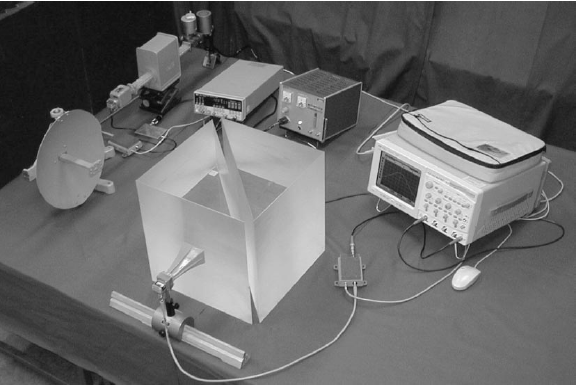
\includegraphics[width=.5\textwidth]{Prisma-foto}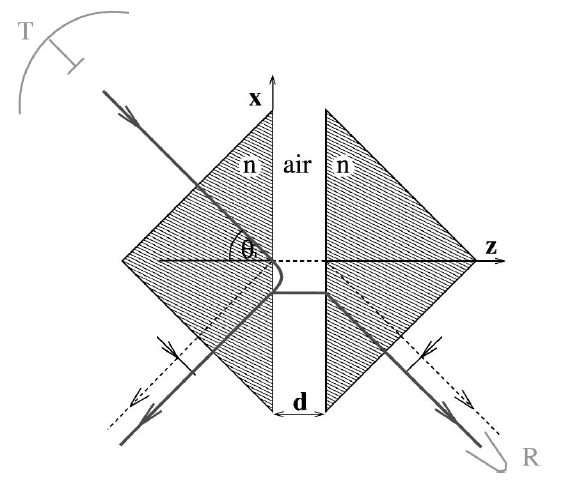
\includegraphics[width=.4\textwidth]{Prisma-zeichnung}    
    \end{itemize}
\end{frame}

    
\input{finalframe.inc}
   
\end{document}